\subsection{Problem formulation}
\label{method1}
We follow the formulation of procedure planning in instructional videos as outlined by \citet{chang2020procedure}. As illustrated in Figure \ref{fig:task}, given an initial visual observation $V_{start}$ and a target visual observation $V_{goal}$, both are short video clips indicating different states of the real-world environment extracted from an instructional video, the model's objective is to generate a sequence of actions $a_{1:T}$ that transitions the environment from $V_{start}$ to $V_{goal}$. Here, $T$ denotes the planning horizon, representing the number of action steps required, while ${V_{start}, V_{goal}}$ define two distinct states of the environment in an instructional video. We use $a_t$ to denote the action step at the timestamp $t$, and in the following, $V_s$ and $V_g$ are short for $V_{start}$ and $V_{goal}$. 

% We use at to denote the action step at the timestamp
% t, and in the following, vs and vg are short for vstart and
% vgoal. Mathematically, the procedure planning problem is
% defined as p (a1:T |vs, vg) that denotes the conditional prob￾ability distribution of the action sequence a1:T given the ini￾tial visual observation vstart and the goal visual state vgoal.

Mathematically, this problem can be formulated as $p(a_{1:T} \mid V_{s}, V_{g})$. Following \citet{wang2023pdpp}, we decompose procedure planning into three sub-problems, as outlined in \cref{eq:1}. The first sub-problem entails learning task-related information $c$ from the observation pair ${V_{s}, V_{g}}$, serving as the initial inference step. The second sub-problem focuses on reconstructing latent visual features. Prior work \citep{wang2023pdpp, bi2021procedure} has approached this by either leveraging long-horizon information \citep{bi2021procedure} or improving sample efficiency \citep{wang2023pdpp}. Considering the lack of intermediate visual observations supervisions, we hypothesize that getting them from other way can especially enhance the coherence of temporal logic. Therefore, we introduce latent temporal interpolations $\upsilon_{1:n}$ to reveal hidden temporal and logical structures within the action sequences, where $n$ represents the number of latent frames to interpolate. The final sub-problem involves generating action sequences based on the task information and visual observations.
\begin{equation} 
p(a_{1:T} \mid V_{s}, V_{g}) = \iint p(a_{1:T} \mid \upsilon_{1:n}, c, V_{s}, V_{g}) p(\upsilon_{1:n} \mid V_{s}, V_{g}) p(c \mid V_{s}, V_{g}) d\upsilon_{1:n} dc .
\label{eq:1} \end{equation}
\begin{figure}[ht]
\centering
% \vspace{0.2em} % 增加上方空白
% \hspace{1em} % 增加左方空白
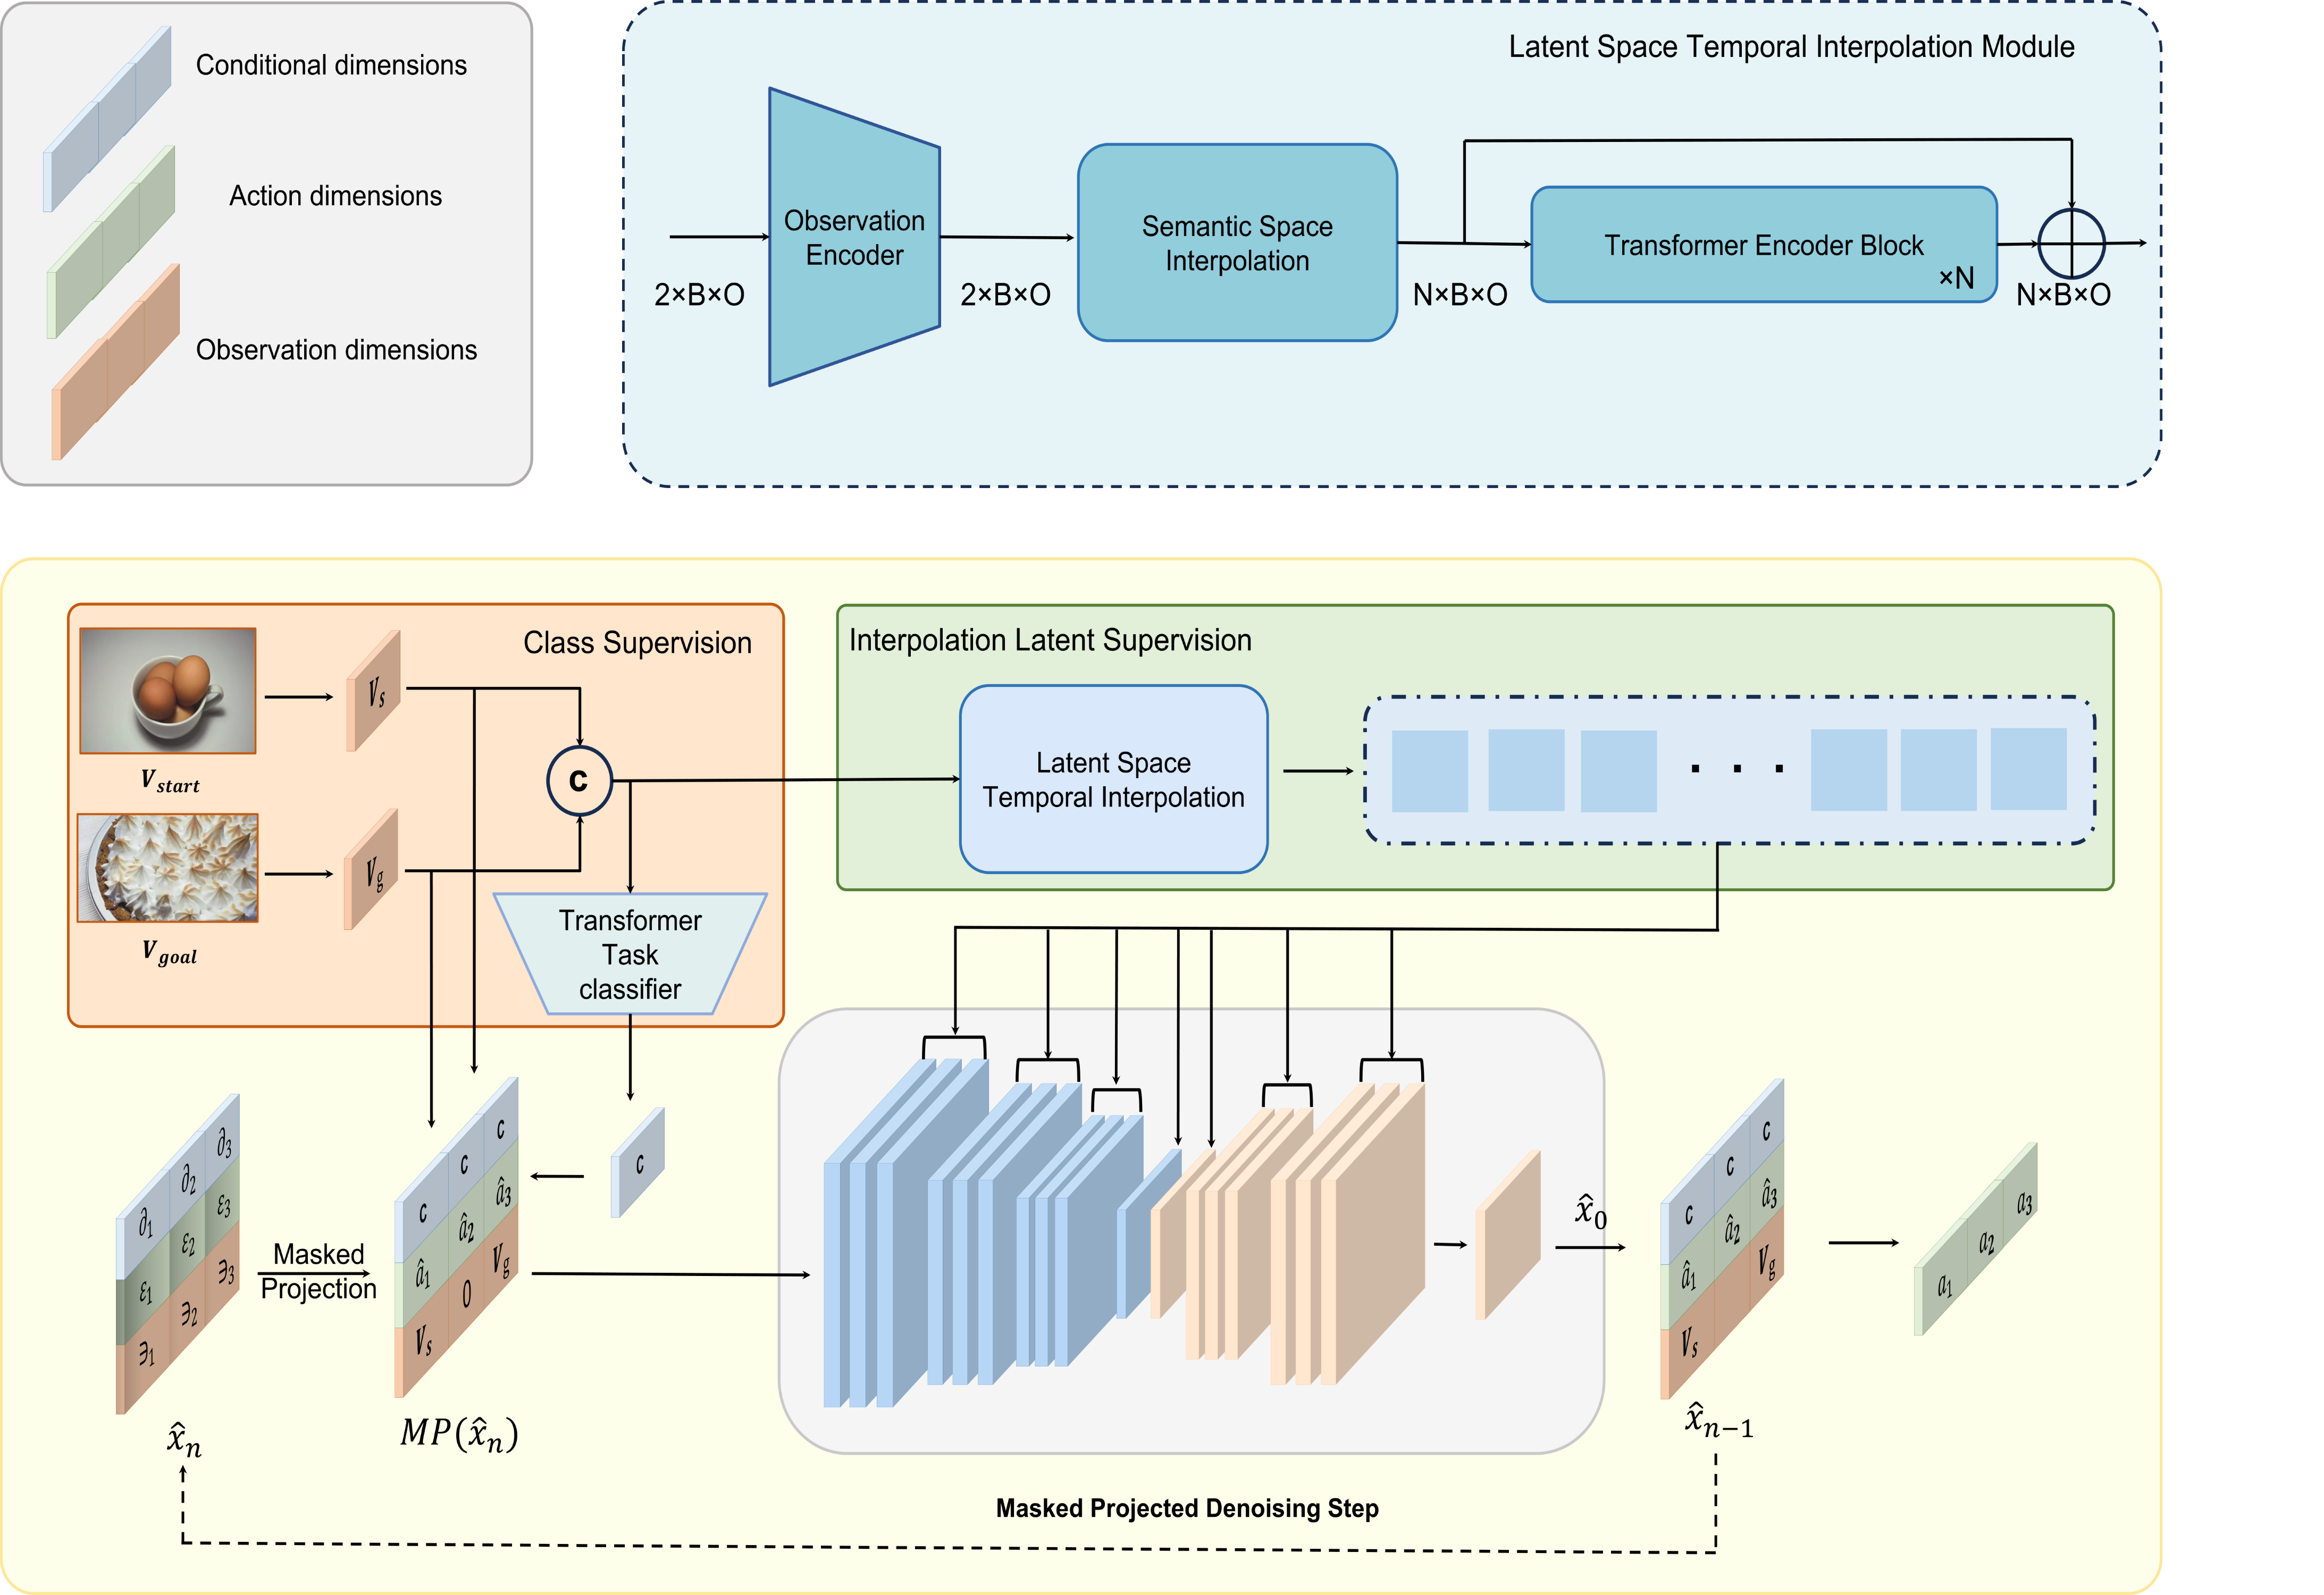
\includegraphics[width=1.06\textwidth, height=0.39\textheight]{figures/architecture.png}
% \hspace{1em} % 增加右方空白
% \vspace{-0.5em} % 增加下方空白
\caption{Overview of our masked temporal interpolation diffusion (prediction horizon $T=3$). We first train a transformer task classifier to generate condition information $c$, which will be used as guidance along with the given observations $V_s$ and $V_g$. Sequentially, we put the concatenated observations into latent space temporal interpolation module to obtain the latent temporal and logic supervision. Then we compute the denoising process iteratively. In each step, we first conduct a masked projection to the input, then predict the initial distribution by the learned model $f(\theta)$. After that we calculate $\hat{x}_{n-1}$ with the U-Net output $\hat{x}_0$. We finally select the action dimensions as our result after $N$ denoising steps. }
\label{fig:architecture}
\end{figure}

During training, we first use a transformer encoder to predict task labels $c$ from observation pairs ${V_{s}, V_{g}}$. The predicted task categories from the instructional videos supervise the model. Next, a temporal interpolation module maps $V_{s}$ and $V_{g}$ into the latent space, filling in the latent frames to guide a U-Net model in learning temporal and logical relationships between actions. During inference, we generate action sequences $a_{1:T}$ by sampling from the learned distribution based on the start and goal observations and the predicted task $c$.
